\documentclass[border=8pt]{standalone}
\usepackage[T1]{fontenc}
\usepackage{xcolor}
\usepackage{amsmath}
\usepackage{siunitx}
\usepackage{tikz}
\usetikzlibrary{arrows.meta,positioning,shapes.geometric,calc,fit,backgrounds}
\usepackage[siunitx,american]{circuitikz}
\usepackage{mathptmx}
\definecolor{ink}{HTML}{14202B}
\definecolor{slate}{HTML}{24394B}
\definecolor{amber}{HTML}{C9781E}
\definecolor{amberlight}{HTML}{FBEBD3}
\definecolor{teal}{HTML}{3E7F8C}
\definecolor{paper}{HTML}{F6F3EC}
\definecolor{muted}{HTML}{5E6974}

\newcommand{\code}[1]{\texttt{#1}}
\tikzset{
  blk/.style={draw=slate,rounded corners=3pt,fill=white,align=center,font=\small,minimum height=0.9cm,text width=3.3cm},
  hub/.style={draw=amber,line width=1.1pt,rounded corners=4pt,fill=amberlight,align=center,font=\small},
  arr/.style={-{Stealth[length=2.2mm]},draw=slate,line width=0.7pt},
  stp/.style={draw=slate,rounded corners=3pt,fill=white,align=center,font=\small,minimum height=1.1cm,text width=4.2cm},
}

\begin{document}
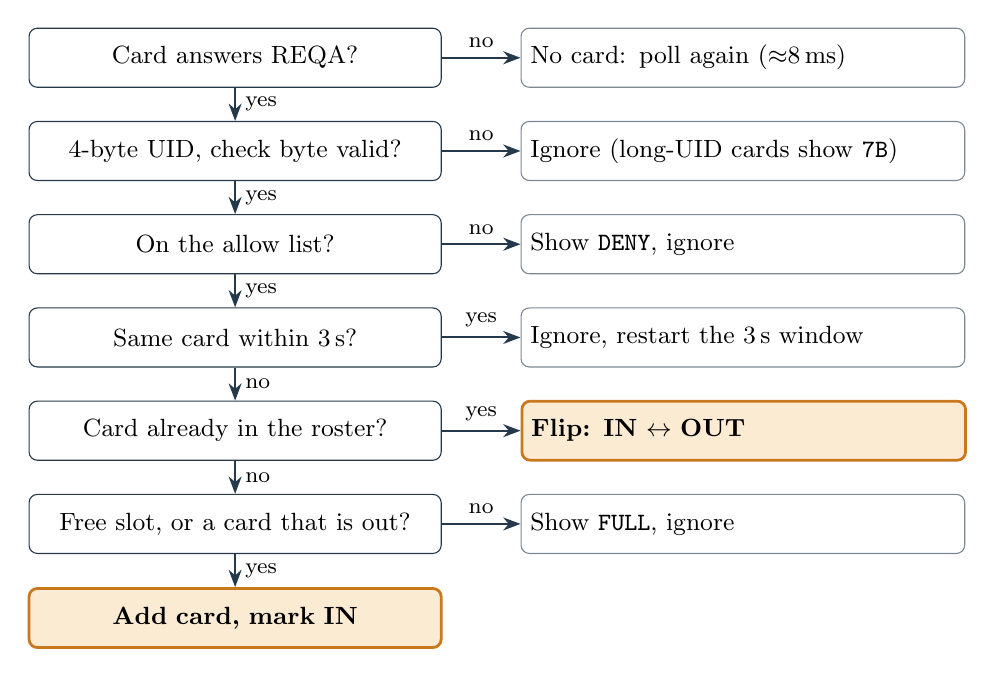
\begin{tikzpicture}[node distance=0.42cm and 1.0cm,
  q/.style={draw=slate,rounded corners=3pt,align=center,font=\small,text width=5.0cm,minimum height=0.75cm},
  res/.style={draw=slate!60,rounded corners=3pt,align=left,font=\small,text width=5.4cm,minimum height=0.75cm},
  good/.style={q,draw=amber,line width=1pt,fill=amberlight}]
\node[q] (a) {Card answers REQA?};
\node[q,below=of a] (b) {4-byte UID, check byte valid?};
\node[q,below=of b] (c) {On the allow list?};
\node[q,below=of c] (d) {Same card within 3\,s?};
\node[q,below=of d] (e) {Card already in the roster?};
\node[q,below=of e] (f) {Free slot, or a card that is out?};
\node[good,below=of f] (g) {\textbf{Add card, mark IN}};
\node[res,right=of a] (xa) {No card: poll again ($\approx$8\,ms)};
\node[res,right=of b] (xb) {Ignore (long-UID cards show \code{7B})};
\node[res,right=of c] (xc) {Show \code{DENY}, ignore};
\node[res,right=of d] (xd) {Ignore, restart the 3\,s window};
\node[res,right=of e,draw=amber,line width=1pt,fill=amberlight] (xe) {\textbf{Flip: IN $\leftrightarrow$ OUT}};
\node[res,right=of f] (xf) {Show \code{FULL}, ignore};
\foreach \u/\v/\l in {a/b/yes,b/c/yes,c/d/yes,d/e/no,e/f/no,f/g/yes} \draw[arr] (\u) -- node[right,font=\footnotesize]{\l} (\v);
\foreach \u/\v/\l in {a/xa/no,b/xb/no,c/xc/no,d/xd/yes,e/xe/yes,f/xf/no} \draw[arr] (\u) -- node[above,font=\footnotesize]{\l} (\v);
\end{tikzpicture}
\end{document}
